\subsection{Regions}

First of all we began by filtering our dataset as soon as the App begins to load so that further ahead when we need the data for the selected region it's already filtered. For this purpose we used the \verb!reactiveVal()! function to create eight {\sf{reactive value}} objects. One for each region and another one for the whole country. The package used for this endeavour was the \verb!dplyr! package and was used as follows:
\begin{itemize}
\item We begin by creating the reactive object:

\begin{verbatim}
loaded_Alentejo <- reactiveVal()
\end{verbatim}

\item And end by loading it with the filtered data:

\begin{verbatim}
Alentejo <- loadedData2() %>% filter(Region == "PTCSR01")
loaded_Alentejo(Alentejo)
\end{verbatim}

Where \verb!loadedData2()! is the data for the whole country.
\end{itemize}
Having done this and in order to know the selected region tab, we gave an id to the Regions tab upon drawing our User Interface so that at the point of which we started to manipulate our data we would know the region we were dealing with. 

\subsubsection{Administered vaccines by week}

We begin by clearing the dataset of the unnecessary columns for the graphic. After this we are left with four columns: \verb!YearWeekIS0!, \verb!FirstDose!,
\\
\verb!SecondDose! and \verb!Vaccine!. 
\\
Having done this we'll need to add the doses of every vaccine available in each and every week and place all those values in an array. What we mean by this is: If a week has 4 reports, each relative to a certain type of vaccine, we'll need to add every First and Second Dose of all those four types and associate that sum to the week.
Finally we create a data-set with the Dates and with the Doses, and since we are taking care of this data with the reactive function, when we call such function in the renderPlot we'll receive the data-set.

In the renderPlot function all we'll have to do is give the ggplot function, from the ggpplot2 package, the data-frame, the aesthetic mappings of the contents of the data-frame, and add geom\_bar() with stat='identity' so that ggplot2 knows that we'll provide the y values. Here's an example on how that would look like:

\begin{verbatim}
output$yourPlotID <- renderPlot({

  res <- myReactiveDat()      ## the data-frame

  ggplot(res, aes(x=Data, y= Doses,fill=Doses)) +  
    geom_bar(stat='identity')+ 
    scale_fill_gradient(low="#63ACAA",high="#507D94")+          ##visual settings
    theme(axis.text.x = element_text(angle = 45, vjust = 0.5), 
          axis.title = element_text(face="bold", size=18),
          title = element_text(size = 20)) + 
    xlab('Week') +
    ylab('Doses')
})
\end{verbatim}

Here's how this graphic would look like (\ref{fig:diagrama}):

\begin{figure}[H]
\centering
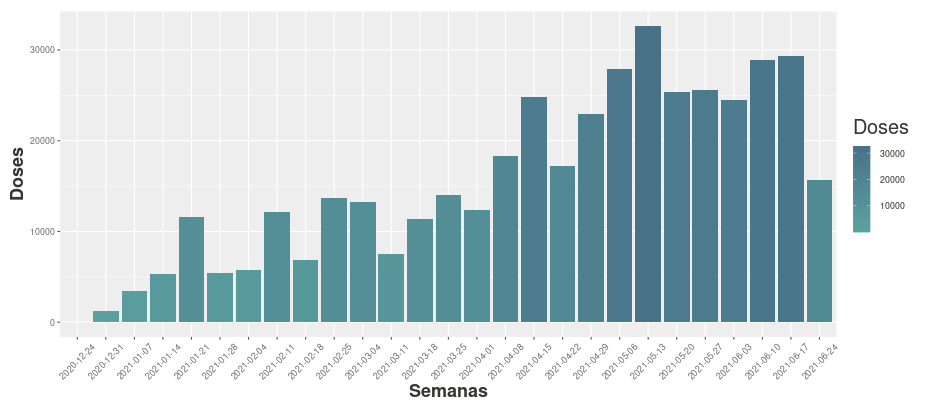
\includegraphics[width=300pt,trim=10 0 0 -10mm]{images/grafico1novo.png}
\caption{Administered vaccines by week}
\label{fig:diagrama}
\end{figure}

\subsubsection{Cumulative value of vaccines by week}

This graphic will follow the exact same principle of the previous one, however, this time we'll have to apply the "cumsum" function from RStudio to our Doses vector. This function returns a vector whose elements are the cumulative sums of the elements of the argument and was used as follows:

\begin{verbatim}
output$yourPlotID <- renderPlot({
  
  res <- myReactiveDat()
  
  (ggplot(res, aes(x=Data, y=cumsum(Doses),group=1))
    + geom_line(color="#63ACAA")
    + geom_point(color="#507D94") 
    + theme(axis.text.x = element_text(angle = 45, vjust = 0.5),
            axis.title = element_text(face="bold", size=18),
            title = element_text(size = 20))  
    + xlab('Week') 
    + ylab('Doses')
    
  )
})
\end{verbatim}

As you can see, the data used is the same as the one in the first graphic, except for the fact that we'll apply the function to the 'Doses' vector.
And since we're trying to see the progress we use the geom\_line function as well as the geom\_point function for a better perception of the results.


Here's how this graphic would look like (\ref{fig:diagrama1})
\begin{figure}[H]
\centering
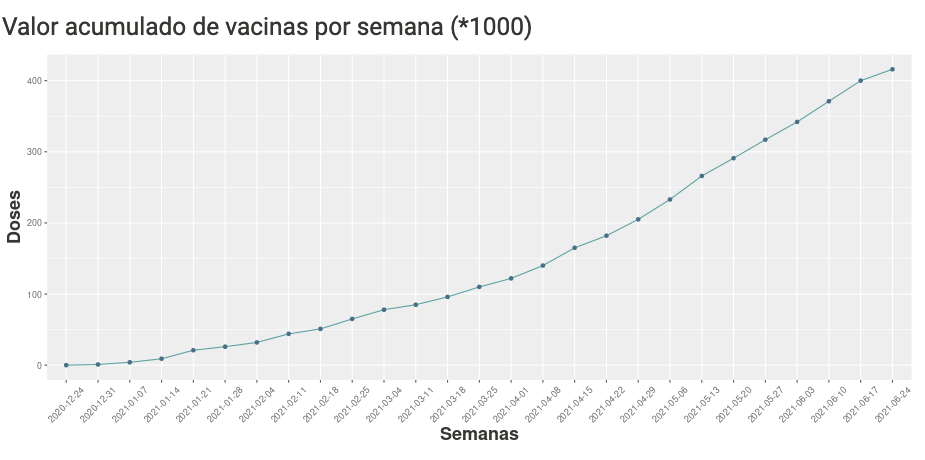
\includegraphics[width=300pt,trim=10 0 0 -10mm]{images/grafico2novo.png}
\caption{Cumulative value of vaccines by week}
\label{fig:diagrama1}
\end{figure}

\subsubsection{Percentage: Vaccinated/Incomplete Vaccination}

For this chart we had to pay careful attention to the data for each region since there are certain Vaccine brands that are yet to be administered in some regions. Having this in consideration and the vaccination treatment of each vaccine, the procedure to find the intended values to draw the waffle chart will consist in getting the sum of all the Second Doses from Moderna, Pfizer and AstraZeneca vaccines and adding the sum of all the First Doses of the Jansen vaccine. This total will be the amount of people that are completely vaccinated and if we subtract it from the population of the region we'll get the amount of people that haven't completed the full vaccination treatment.

After getting both values, in order to get the percentages, all we had to do was dividing both numbers by the region population and multiplying the result by 100. Then we create a vector with both percentages and since we're working on this data with the reactive function, when we call it we'll receive said vector.

Finally we draw our Waffle chart (\ref{fig:diagrama2})
\begin{verbatim}
output$yourPlotID <- renderPlot({
  resWaffle <- myReactiveWaffles()
  val_names <- sprintf("%s (%s%%)", 
                       c("Vacinação incompleta: ", 
                         "Completamente Vacinados: "), 
                       resPie)
  names(resWaffle) <- val_names
  waffle::waffle(resPie)
})
\end{verbatim}

\begin{figure}[H]
\centering
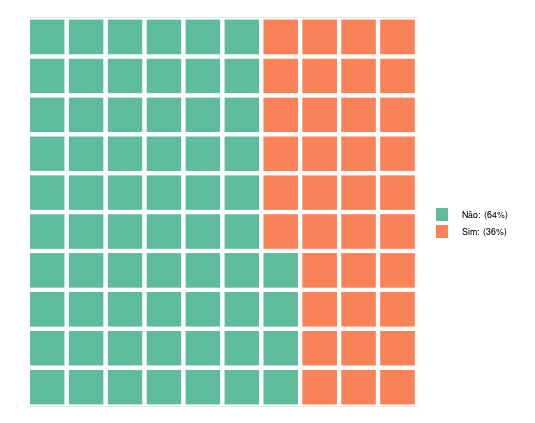
\includegraphics[width=300pt,trim=10 0 0 -10mm]{images/graficomapa2.png}
\caption{Percentage: Vaccinated/Incomplete Vaccination}
\label{fig:diagrama2}
\end{figure}

\subsubsection{Administered vaccines by laboratory}

We start off by filtering the data for every vaccine. After this we'll need to verify whether the data frame of each vaccine is not empty just in case the region we're dealing with has not received any vaccines of that laboratory. If the data frames are not empty, we'll create a variable for each one with the sum of both the First Doses as well as the Second Doses. At last a vector with these values is created so that, when we call the reactive function in the renderPlot, we can access this data.

Here's how the renderPlot function would look like:

\begin{verbatim}
output$yourPlotID <- renderPlot({
  
  res <- VacinasReg()
  ggplot(res, aes(x=Nomes, y=Totais, fill = c6)) + 
    geom_bar(stat='identity')+ 
    scale_fill_manual(values = c("AZ"="#D8BFD8",
                                 "MOD"="#B0E0E6",
                                 "COM"="#FFDAB9",
                                 "JJ"="#c6ffb3")) +
    geom_text(aes(label=Totais), vjust = -0.6, size = 4)+
    theme(
      legend.position = "none",
      axis.text.x = element_text(angle = 20, vjust = 0.5),
      axis.title = element_text(face="bold", size=18),
      axis.text.y = element_blank(),
      axis.ticks.y = element_blank(),
      title = element_text(vjust = 1, size = 20),
      panel.grid = element_blank(),
      panel.background = element_rect(fill ="#ffffff")
    ) + 
    xlab('') +
    ylab('') 
})
\end{verbatim}

As we can see, the res variable will consist of a data frame with both the names of the vaccines as well as the totals. Knowing this, the process to draw the graphic is more or less the same as most of the others. We pass these values onto the ggplot function and after that we add the geom\_bar in order to draw an bar plot (\ref{fig:diagrama3}). 

\begin{figure}[H]
\centering
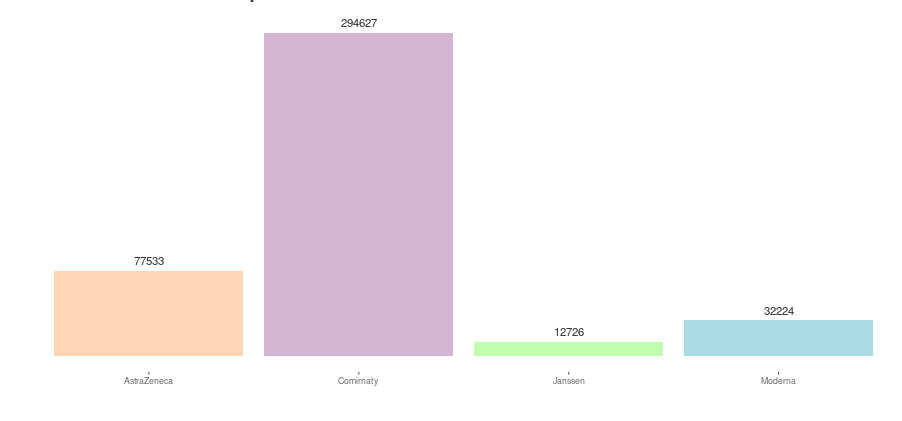
\includegraphics[width=300pt,trim=10 0 0 -10mm]{images/grafico4novo.png}
\caption{Administered vaccines by laboratory}
\label{fig:diagrama3}
\end{figure}